\section{実データ解析}
本章では実データを解析する.
本章では「NMF1回の結果」は「初期値を100回変えてNMFを行い目的関数が最小となった結果」とする.

\subsection{実データ}
本研究で用いるデータは筑波大学の柳沢研究所で計測されたカルシウムイメージングデータである.
本データは,2光子多細胞カルシウムイメージングによって1匹のマウスの大脳皮質1次運動野第2・3層のニューロンのイメージング画像を得た後,人手でROIがつけられ,ニューロンごとの数値データに直されたものである.
1時間おきに15分間のイメージングが計6回行われ,各イメージングのサンプリングレートは8[Hz]である.
このサンプリングレートは使用された機器の最大のものである.
用いられた蛍光タンパク質はGCaMP6sである.
実験系は\Figref{fig:imaging}(A)の系で行われた\cite{Kanda2016}.
観測されたニューロン数は154であった.
時間方向には4[s]ごとのマウスの状態(wake, REM, NREM)のラベルが付いており,ニューロンごとに興奮性か抑制性のラベルがついている.
\Figref{fig:wholedata}にニューロン3つの時系列と時系列方向についているラベル(wake,NREM,REM)を示す.

\begin{figure}[htbp]
    \begin{center}
				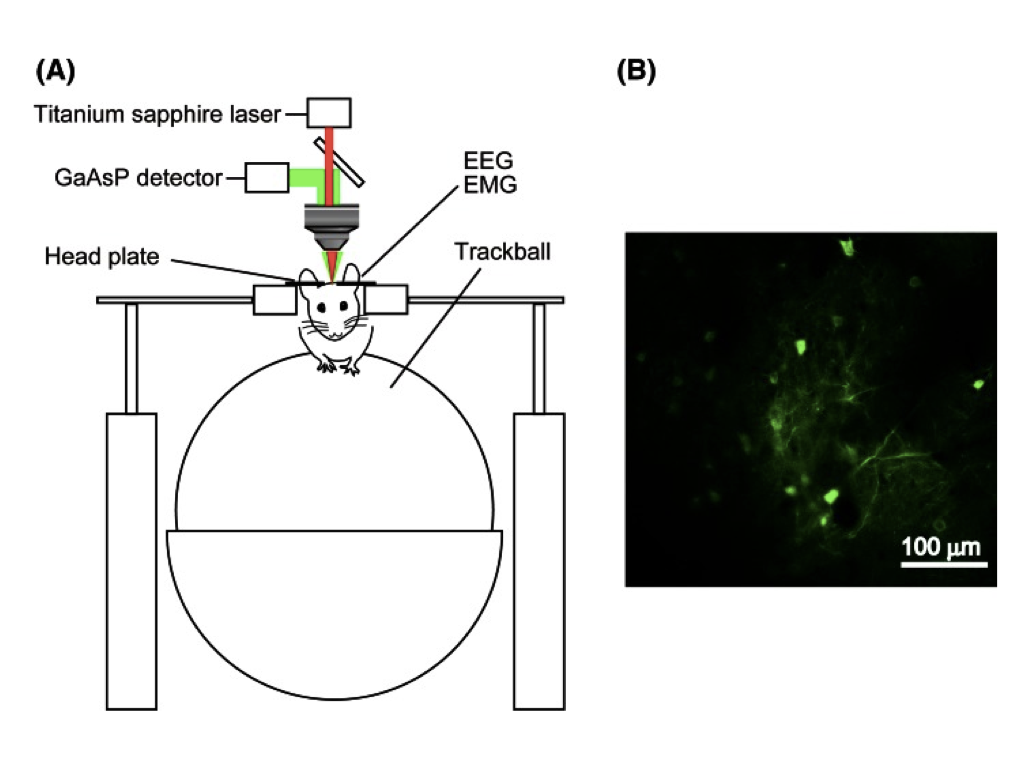
\includegraphics[width=0.8\linewidth]{imaging}
				\caption{(A)カルシウムイメージングの測定系.マウスは頭を固定されたままボールの上で活動することができる.(B)カルシウムイメージング画像.}
        \label{fig:imaging}
    \end{center}
\end{figure}

\begin{figure}[htbp]
	\begin{center}
		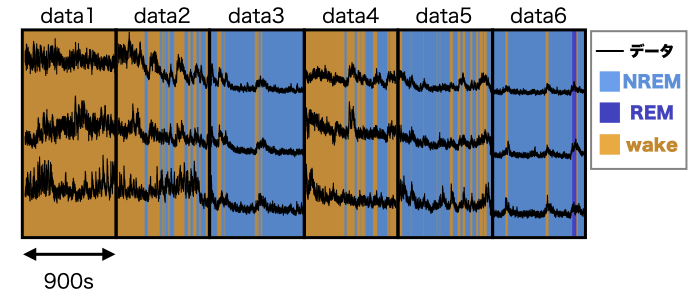
\includegraphics[width=\hsize]{datawhole}
	\end{center}
	\label{fig:wholedata}
\end{figure}

\subsection{実験設定}
6回計測されたデータそれぞれについてクラスタリングを行う.
NMFを一回行,それを最尤推定の結果とする.
最尤推定結果からBICを計算し,目視で基底数の範囲を決める.
範囲内の基底数について100回ブートストラップを行い,$\bar{A}$を求める.
固有値ギャップを算出し,スペクトラルクラスタリングを行う.

\subsection{結果}
推定されたクラスタを\Figref{fig:real-clst}に示す.

\begin{figure}[htbp]
    \begin{minipage}{0.32\hsize}
			\begin{center}
					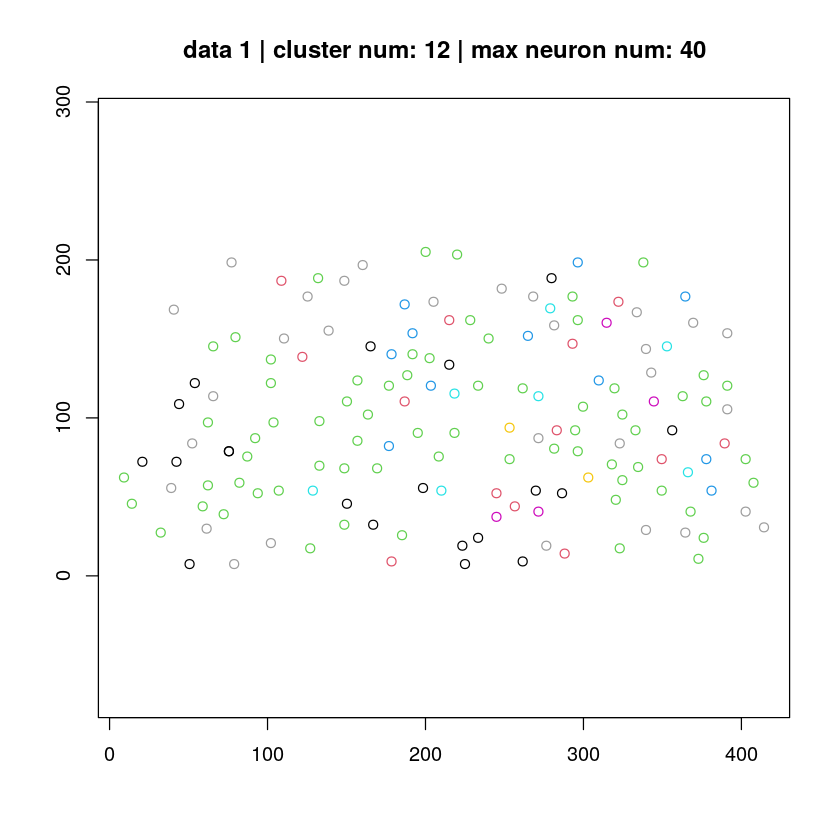
\includegraphics[width=\hsize]{cluster1}
			\end{center}
		\end{minipage}
    \begin{minipage}{0.32\hsize}
			\begin{center}
					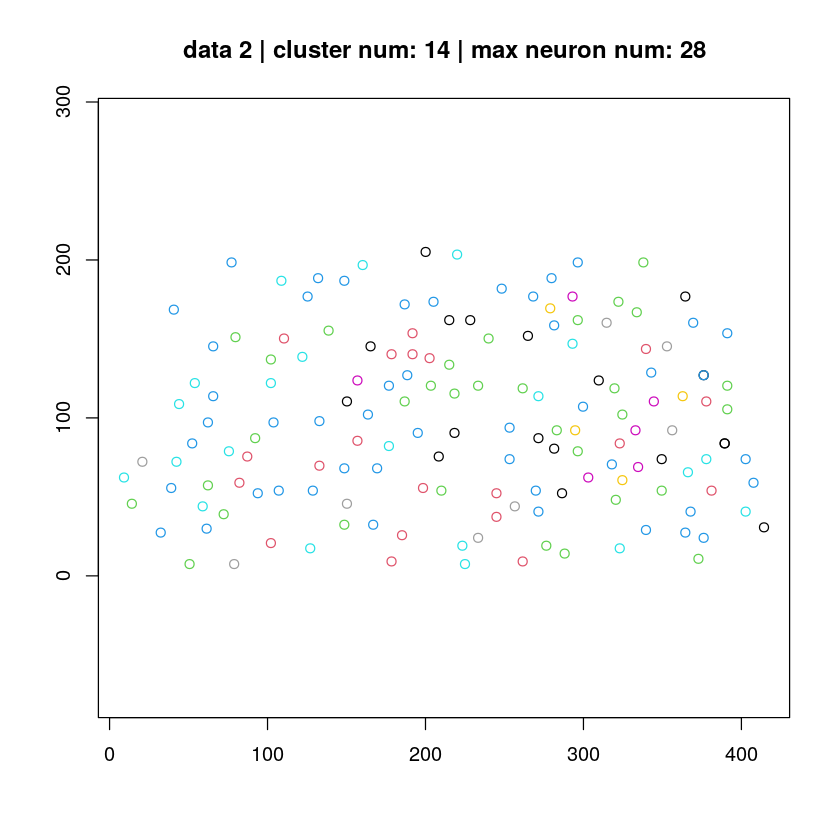
\includegraphics[width=\hsize]{cluster2}
			\end{center}
		\end{minipage}
    \begin{minipage}{0.32\hsize}
			\begin{center}
					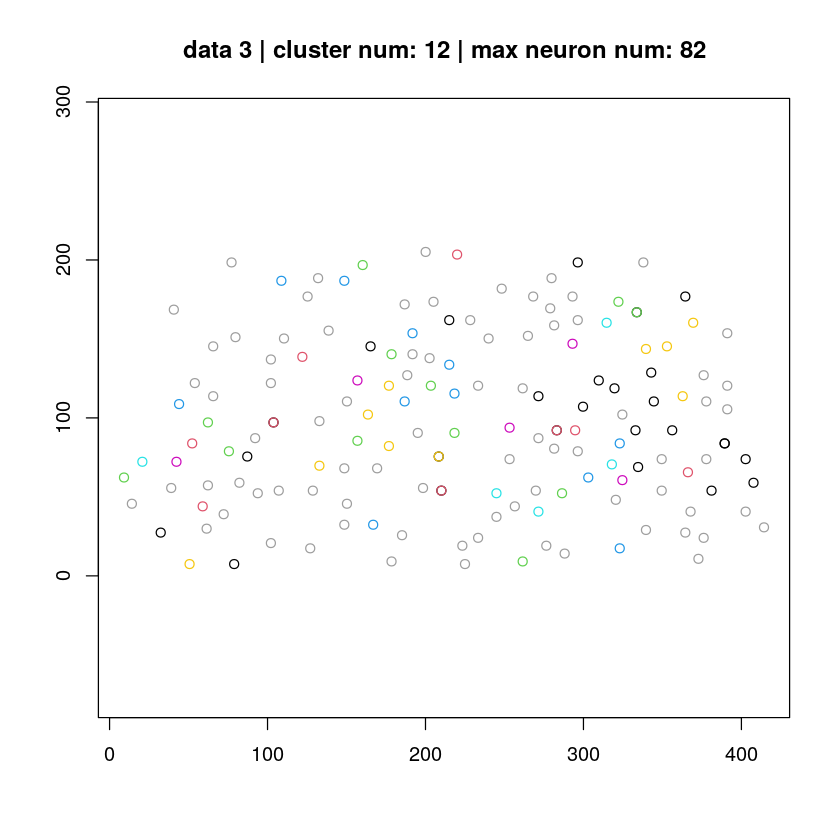
\includegraphics[width=\hsize]{cluster3}
			\end{center}
		\end{minipage}\\
    \begin{minipage}{0.32\hsize}
			\begin{center}
					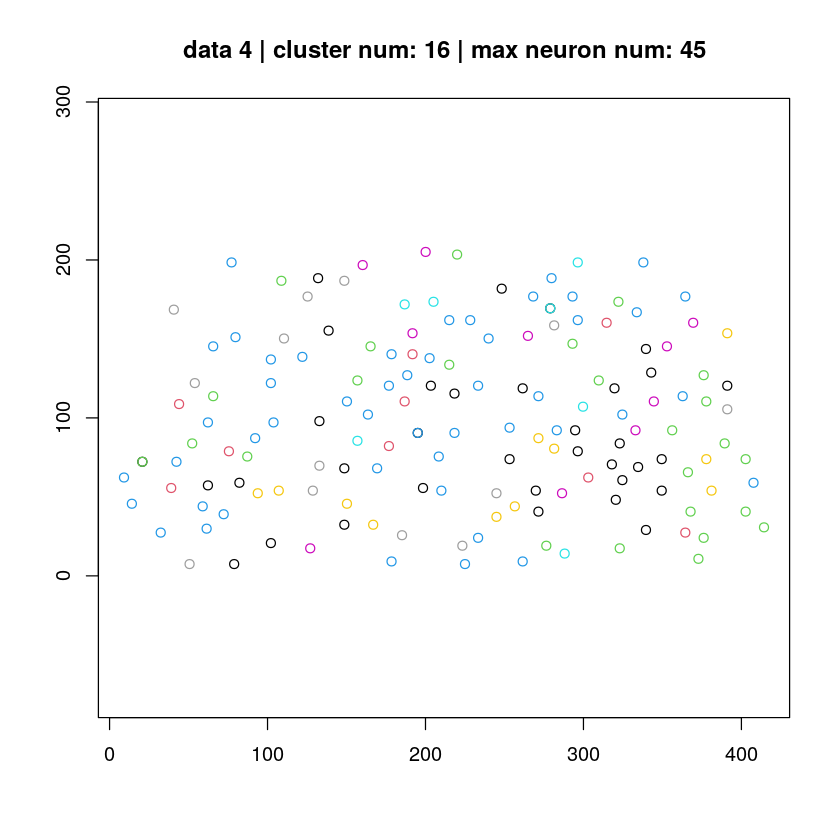
\includegraphics[width=\hsize]{cluster4}
			\end{center}
		\end{minipage}
    \begin{minipage}{0.32\hsize}
			\begin{center}
					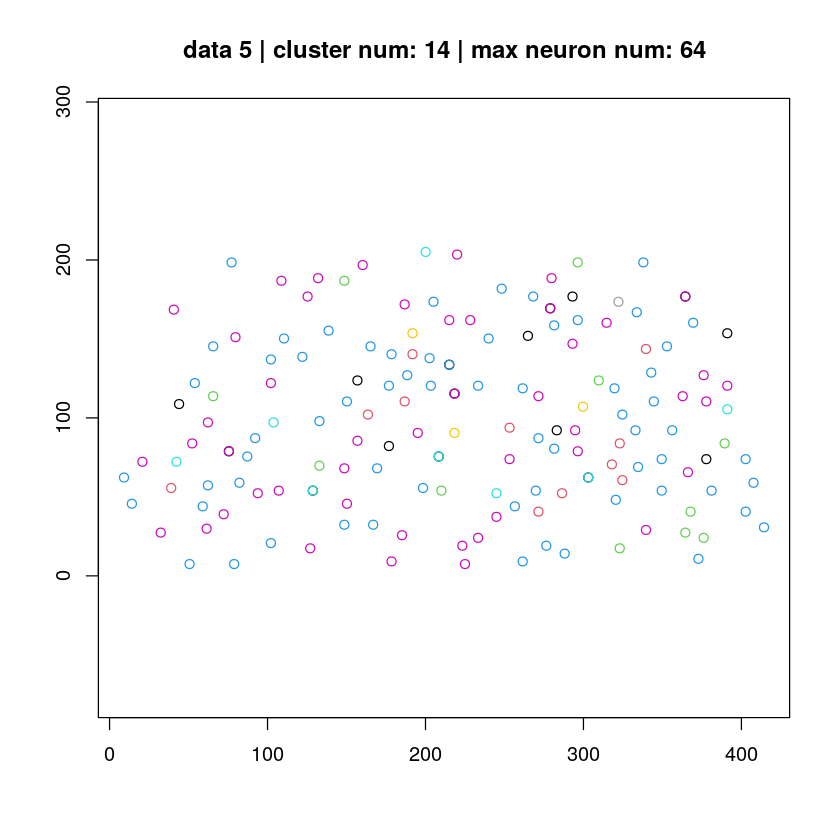
\includegraphics[width=\hsize]{cluster5}
			\end{center}
		\end{minipage}
    \begin{minipage}{0.32\hsize}
			\begin{center}
					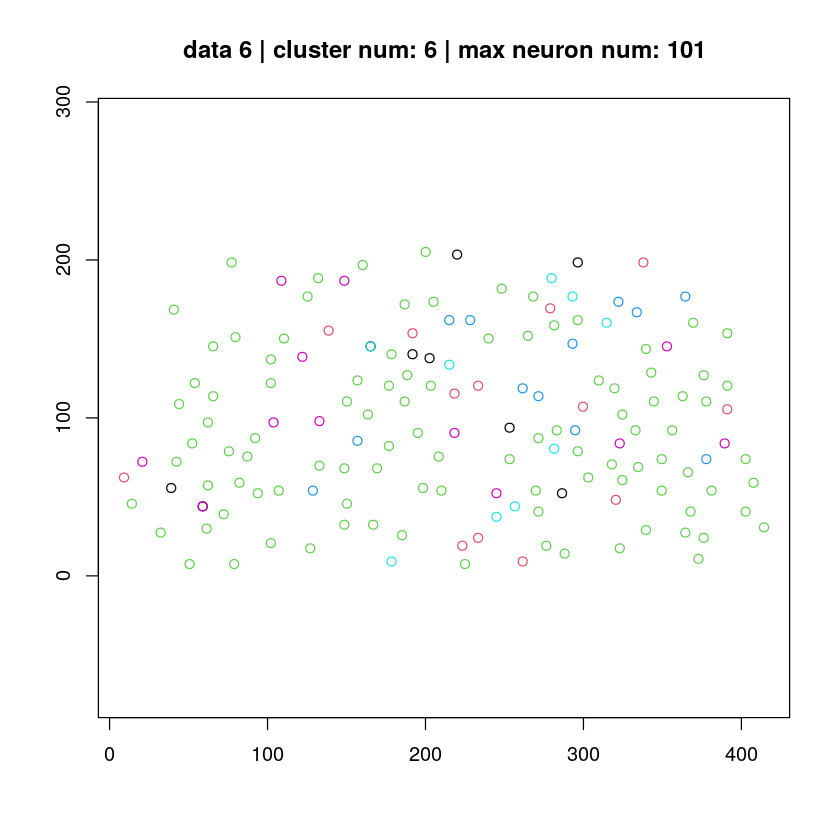
\includegraphics[width=\hsize]{cluster6}
			\end{center}
		\end{minipage}
		\label{fig:real-clst}
\end{figure}
